% Beamer slide template prepared by Tom Clark <tom.clark@op.ac.nz>
% Otago Polytechnic
% Dec 2012

\documentclass[10pt]{beamer}
\usetheme{Dunedin}
\usepackage{graphicx}
\usepackage{fancyvrb}

\newcommand\codeHighlight[1]{\textcolor[rgb]{1,0,0}{\textbf{#1}}}

\title{Network Sockets 1}

\author[IN608]{Intermediate Application Development}
\institute[Otago Polytechnic]{
  Otago Polytechnic \\
  Dunedin, New Zealand \\
  Kaiako: Tom Clark
}
\date{}
\begin{document}

%----------- titlepage ----------------------------------------------%
\begin{frame}[plain]
  \titlepage
\end{frame}

%----------- slide --------------------------------------------------%
\begin{frame}
  \frametitle{Introduction}
  
  Today it seems like just about any application we write involves some
  degree of network interaction. Our processes communicate with each other 
  using \emph{network sockets}.
  
  These sockets are really just one (very common) form of interprocess communication.
  The general principles we apply in this case apply across  interprocess communiction
  in general.
  
  \end{frame}

%----------- slide --------------------------------------------------%
\begin{frame}
  \frametitle{Network model}
  
  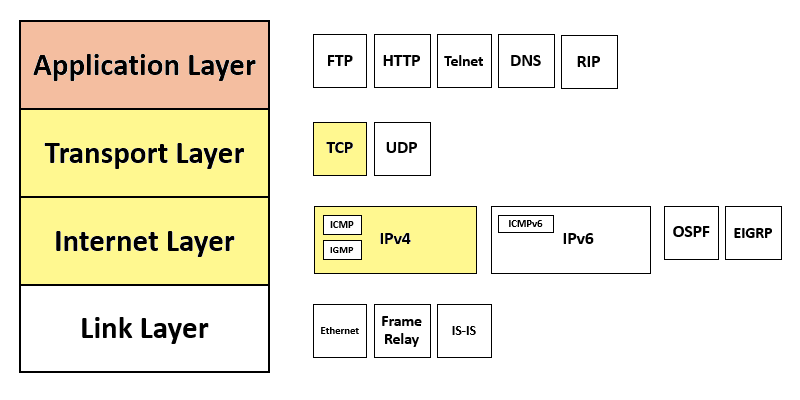
\includegraphics[width=8cm]{tcp-ip.png}
  
  {\tiny image: Michel Bakni (\url{https://www.wikidata.org/wiki/Q81411358})}  
  \end{frame}

%----------- slide --------------------------------------------------%
\begin{frame}
  \frametitle{Servers and clients}
  
  We will discuss writing both client and server applications. For
  our purposes
  
  \begin{itemize}
    \item A \emph{server} application listens for incoming requests and responds to them;
    
    \item A \emph{client} initiates communication by opening a connection to a server.
  \end{itemize}
  
  A particular application may act like a server at some times and like a client at other times. 
    
  \end{frame}

%----------- slide --------------------------------------------------%
\begin{frame}
  \frametitle{Network socket flow}
  
   
  \begin{enumerate}
    \item The server creates a socket.
    \item The server binds the socket to an address/port.
    \item The server listens for connections to the socket.
    \item The client creates a socket.
    \item The client connects to the server's socket.
    \item the server accepts the client connection.
    \item The client and server send and receive data.
    \item The client closes its connection, notifying the server.
    \item The server closes its connection.
   \end{enumerate}
  
  
    
  \end{frame}

%----------- slide --------------------------------------------------%
\begin{frame}[fragile]
  \frametitle{In code}
  
  \begin{verbatim}
  # Server:                                                                                                       
  import socket                                           
  s = socket.socket(socket.AF_INET, socket.SOCK_STREAM)  # 1
  s.bind(('127.0.0.1', 65432))                           # 2
  s.listen()                                             # 3
  conn, addr = s.accept()                                # 6
  data = conn.recv(1024)                                 # 7.2
  conn.sendall(b'received')                              # 7.3
  data = conn.recv(1024)                                 # 8.2
  conn.close()                                           # 9
  
  # Client 
  import socket
  s = socket.socket(socket.AF_INET, socket.SOCK_STREAM)  # 4
  s.connect(('127.0.0.1', 65432))                        # 5
  s.sendall(b'Hello')                                    # 7.1
  data = s.recv(1024)                                    # 7.4
  s.close()                                              # 8.1
  \end{verbatim} 
   
\end{frame}
%----------- slide --------------------------------------------------%
\begin{frame}
  \frametitle{Programming Activity}
  
  \begin{enumerate}
    \item Pull the course materials repo.
    \item Create a new branch, \texttt{19-practical} in your practicals repo.
    \item Copy the subdirectory, \texttt{19-practical} from the class materials into your repo.
    \item See the README for directions.
    \item We will discuss results in 30ish minutes.
  \end{enumerate}      
\end{frame}
  
%----------- slide --------------------------------------------------%
\begin{frame}
  \frametitle{A problem}
  
  Our server can only handle one connection at a time. While it's servicing that
  connection, other clients just queue up and wait. 
  
  \vspace{5mm}
  In particular, calls to \texttt{accept()} and \texttt{recv()} block waiting on 
  data from the socket.
  
  \vspace{5mm}
  Even when we solve this problem, our application code needs some sort of
  concurrency mechanism to handle multiple clients. 
    
\end{frame}

%----------- slide --------------------------------------------------%
\begin{frame}
  \frametitle{Concurrency}
  
  We will cover concurrency in more detail next week, but briefly our options
  are
  \begin{itemize}
    \item Threading
    \item Forking
    \item Asyncio
    \item Select
  \end{itemize}   
  
  We will use select today.   
\end{frame}
%----------- slide --------------------------------------------------%
\begin{frame}[fragile]
  \frametitle{Server: setting up}
  
 
  \begin{verbatim}
  import socket
  import selectors
  ...
  clients = selectors.DefaultSelector()
  listener = socket.socket(socket.AF_INET, socket.SOCK_STREAM)
  listener.bind((host, port))
  listener.listen()
  listener.setblocking(False)
  clients.register(listener, selectors.EVENT_READ, data=None)
  \end{verbatim} 
  Two things are going on here:
  \begin{enumerate}
    \item We use \texttt{setblocking(False)} so that, when we call \texttt{accept()} later,
    our code won't block waiting on a connection.
    \item We register our listener with our selector, telling the selector to notify us if the listener
    receives data.
  \end{enumerate}  
  
   
\end{frame}
%----------- slide --------------------------------------------------%
\begin{frame}[fragile]
  \frametitle{Server: event loop}
  
  Now we basically just loop, waiting for the selector to notify
  us when a client socket has some data to process.
  
  \begin{verbatim}
      while True:
        events = clients.select(timeout=None)
        for event, mask in events:
            if event.data is None:
                accept_connection(event.fileobj, clients)
            else:
                service_connection(event, mask, clients)  
  \end{verbatim} 
  
  When we registered the listener, we set \texttt{data=None}. This is why
  \texttt{event.data} is \texttt{None} for a new connection.
  
   
\end{frame}

%----------- slide --------------------------------------------------%
\begin{frame}[fragile]
  \frametitle{Server: accept connection}
  
 
  
  \begin{verbatim}
  def accept_connection(sock, clients):
      conn, addr = sock.accept()
      conn.setblocking(False)
      data = {'addr': addr, 'buffer': b''}
      events = selectors.EVENT_READ | selectors.EVENT_WRITE
      clients.register(conn, events, data=data)                   
  \end{verbatim} 
  
  Again, notice that we set the connection to be nonblocking once we establish it. We 
  register the newly established connection  with our \texttt{clients} selector.
   
\end{frame}

%----------- slide --------------------------------------------------%
\begin{frame}[fragile]
  \frametitle{Server: service connection}
  
 
  
  \begin{verbatim}
  def service_connection(event, mask, clients):
      sock = event.fileobj
      data = event.data
      if mask & selectors.EVENT_READ:
          recv_data = sock.recv(1024)
          if recv_data:
              data['buffer'] = recv_data
          else:
              client.unregister(sock)
              sock.close()
      if mask & selectors.EVENT_WRITE:
          if data['buffer']:
              sent = sock.sendall(data['buffer'])   
              data['buffer'] = b''          
  \end{verbatim} 
  
  If we received data, we save it in the buffer to send back to the client later. If 
  we're ready to write to client and we have data in buffer, we send it.
   
\end{frame}
%----------- slide --------------------------------------------------%
\begin{frame}
  \frametitle{References}
  
  \begin{itemize}
    \item \texttt{socket} library: \url{https://docs.python.org/3/library/unittest.html}
    \item \texttt{selectors} library: \url{https://docs.python.org/3/library/selectors.html}
    \item RealPython article on socket programming: \url{https://realpython.com/python-sockets/}
  \end{itemize}      
\end{frame}

\end{document}
